\documentclass{article}
\usepackage[utf8]{inputenc}
\usepackage{amsmath}
\usepackage{graphicx}
\usepackage{float}
\usepackage{multibibliography}
\begin{document}

\section*{CV Project \#3}
Name: Qiang Fu
\\Date: December 7th 2019

\subsection*{Introduction} 
Kalman filter is a very classic and effective method to estimate states of a system. In this project we model the feature points tracking problem with a system model and a measurement model and apply the Kalman filter to estimate the 2D coordinates of the feature points. After tracking feature points, we use the factorization method to recover the 3D rotation of the camera and the 3D structure of the feature points.
\subsection*{Theories for the algorithm}
\subsubsection*{Kalman filter}
\par 
The main idea of Kalman filter is to estimate the states of a system by fusing both observation and prediction.
\par
From the lecture notes we know that a linear system can be modeled by two funtions\cite{ref1}
\begin{align}
s_{t+1}&=\Phi s_t+\omega_t
\\z_t &=Hs_t+\epsilon_t
\end{align}
where $\omega_t \sim N(0,Q),\epsilon_t \sim N(0,R)$. Eq.1 is called system model, which shows the relativities between the states at time frame $t$ and time frame $t+1$. The main idea of this equation is that the state of the next time frame can be denoted as a linear combination of current states plus the uncertainty of this model. And Eq.2 is called measurement model, which shows the relativities between the measurements of the system and the inner states at time frame $t$, where the $\epsilon_t$ is the uncertainty of the measurement model. 
\par
What Kalman filter does is to fuse the $z_t$ and $s_{t+1}$ by weighted sum, ant to calculate the weight we have 4 steps.
\begin{enumerate}
\item predict $s_t$ based on state model
\par
Based on the state model, we can calculate the state of the current time frame $s_t$ given the states of the last time frame $s_{t-1}$ by
\begin{equation}
s_{t}^-=\Phi s_{t-1}
\end{equation}
And the uncertainty of this prediction is
\begin{equation}
\begin{split}
\Sigma_t^-&=E\left[ (s_t-s_t^-)(s_t-s_t^-)^T\right]
\\&=\Phi\Sigma_{t-1}\Phi^T+Q
\end{split}
\end{equation}
where $\Sigma_{t-1}$ is the covariance matrix of the final estiamtion of the last time frame.
\item implement observation 
\par
The observation can be written as
\begin{equation}
z_t = Hs_t
\end{equation}
In this project the observation is 2D image coordinates of the feature points from the feature detector using the SSD method. Thus the $H$ matrix is as follow
\begin{equation}
H = \begin{bmatrix}
1&0&0&0\\
0&1&0&0
\end{bmatrix}
\end{equation}
\item fuse the prediction and measurement to produce the final estimated $s$
\par
The final estimation of the states $s_t^*$ can be written the weighted sum of $s_t^-$ and $z_t$
\begin{equation}
s_t^*=s_t^-+K_t(z_t-Hs_t^-)
\end{equation}
And the covariance matrix of $s_t^*$ is
\begin{equation}
\Sigma_t=E\left[(s_t-s_t^*)(s_t-s_t^*)^T\right]=(I-K_tH)\Sigma_t^-
\end{equation}
What we need is the $K$ that minimize the trace of the covariance matrix
\begin{equation}
K_t^*=arg\,\min_{K_t}trace(\Sigma_t)
\end{equation}
Performing $\frac{\delta trace(\Sigma_t)}{\delta K_t}=0$ yields
\begin{equation}
K_t=\Sigma_t^-H^T(H\Sigma_t^-H^T+R)^{-1}
\end{equation}
\item calculate the incertainty of the final estimation 
\par
At last we need to update the covariance matrix of the current states for the next iteration. From the last step, we have
\begin{equation}
\Sigma_t=(I-K_tH)\Sigma_t^-
\end{equation}
\end{enumerate}
\par 
Before iteration, we need to set up the initial value of $s_0,z_0,Q,R,\Sigma_0$. In this project the states include the 2D coordinates and image velocity of the feature points, which can be obtained by feature detector and calculating the difference of the their coordinates in consequtive 2 frames. And as the iteration goes, the trace of $\Sigma_t$ will converge to a relative small value, thus the initial value of $\Sigma$ is not that important, we can just set it to $\begin{bmatrix}100&0&0&0\\0&100&0&0\\0&0&25&0\\0&0&0&25\end{bmatrix}$. We assume that the states are independent as well as the measurements, then we can set $Q=\begin{bmatrix}16&0&0&0\\0&16&0&0\\0&0&16&0\\0&0&0&16\end{bmatrix},R=\begin{bmatrix}9&0\\0&9\end{bmatrix}$

\subsubsection*{Factorization method}
\par
The factorization method is a method that can recover the camera's rotaion relative to the object frame and the features' 3D coordinates from consequtive iamge frames under othographic projection method and assumption that there is only one rigid 3D motion between the camera and object.
\par
Let $p_{ij}=(c_{ij},r_{ij})$ denotes the $j$th image on the image frame. Let $\bar{c}_i$ and$\bar{r}_i$ be the centroid of the image points relative to the onject frame and let $\bar{P}$ be the 3D points. Let
\begin{align}
\begin{split}
c_{ij}^{'} &= c_{ij}-\bar{c}_i\\
r_{ij}^{'} &= r_{ij}-\bar{r}_i\\
P_j^{'} &= P_j-\bar{P}
\end{split}
\end{align}
And under the orthographic assumption, for the $j$th point on the $i$th frame we have
\begin{equation}
\begin{bmatrix}c_{ij}^{'}\\r_{ij}^{'}\end{bmatrix}=\begin{bmatrix}\boldsymbol{r}_{i,1}\\\boldsymbol{r}_{i,2}\end{bmatrix}P_j^{'}
\end{equation} 
where $\boldsymbol{r}_{i,1}$ and $\boldsymbol{r}_{i,2}$ are the first two rows of the rotation matrix between camera frame $i$ and the object frame. And for N frames we have
\begin{equation}
W = RS
\end{equation}
where $R$ is $2N\times3$ matrix and $S$ is $3\times M$ and 
\begin{align}
R&=\begin{bmatrix}
\boldsymbol{r}_{1,1}\\\boldsymbol{r}_{1,2}\\\vdots\\\boldsymbol{r}_{N,1}\\\boldsymbol{r}_{N,2}
\end{bmatrix}\\
S&=\begin{bmatrix}P_1^{'}&P_2^{'}&\dots&P_M^{'}\end{bmatrix}\\
W&=\begin{bmatrix}c_{11}&c_{12}&\dots&c_{1M}\\
				  r_{11}&r_{12}&\dots&r_{1M}\\
				  c_{21}&c_{22}&\dots&c_{2M}\\
				  r_{21}&r_{22}&\dots&r_{2M}\\
				  \vdots&\vdots&\vdots&\vdots\\
				  c_{N1}&c_{N2}&\dots&c_{NM}\\
				  r_{N1}&r_{N2}&\dots&r_{NM}\\
\end{bmatrix}
\end{align}
According to the rank theorem, $Rank(AB)\leq min(Rank(A),Rank(B))$, the matrix $W$ has a maximum rank of 3. However in reality, due to the noise, $W$ may have a rank more than 3, so we can impose the rank theorem by performing a SVD on $W$
\begin{equation}
W = UDV^T
\end{equation}
\begin{enumerate}
	\item Take the left up $3\times3$ submatrix of $D$ to form the $D^{'}$
	\item Keep the first 3 columns of $U$ and remove the else and form $U^{'}$, which is a $2N\times 3$ matrix.
	\item Keep the first 3 columns of $V$ and remove the else and form $V^{'}$, which is a $M\times 3$ matrix.
\end{enumerate}
\begin{equation}
W^{'}=U^{'}D^{'}V^{'T}
\end{equation}
This $W^{'}$ is close to $W$, but satisfies the rank theorem. And apply SVD to $W^{'}$, we have
\begin{equation}
W^{'}=R^{'}S^{'}=U^{'}D^{'}V^{'T}
\end{equation}
However for any $3\times3$ invertible matrix $Q$, $W^{'}=R^{'}QQ^{-1}S^{'}=U^{'}D^{'}V^{'T}$ is also true. So we can find $Q$ using the constraint that rotation matrix $R$ is an orthonormal matrix
\begin{align}
\begin{split}
\boldsymbol{r}_{i,1}\boldsymbol{r}_{i,1}^T&=1\\
\boldsymbol{r}_{i,2}\boldsymbol{r}_{i,2}^T&=1\\
\boldsymbol{r}_{i,1}\boldsymbol{r}_{i,2}^T&=0
\end{split}
\end{align}
Since $R=R^{'}Q$, we have
\begin{align}
\begin{split}
\boldsymbol{r}^{'}_{i,1}QQ^T\boldsymbol{r}^{'T}_{i,1}&=1\\
\boldsymbol{r}^{'}_{i,2}QQ^T\boldsymbol{r}^{'T}_{i,2}&=1\\
\boldsymbol{r}^{'}_{i,1}QQ^T\boldsymbol{r}^{'T}_{i,2}&=0
\end{split}
\end{align}
And denote $QQ^T$ as $A$, we can set up a linear equation system
\begin{equation}
\begin{bmatrix}
\boldsymbol{r}^{'}_{i,1}\boldsymbol{r}^{'}_{i,1}(1)&\boldsymbol{r}^{'}_{i,1}\boldsymbol{r}^{'}_{i,1}(2)&\boldsymbol{r}^{'}_{i,1}\boldsymbol{r}^{'}_{i,1}(3)\\
\boldsymbol{r}^{'}_{i,2}\boldsymbol{r}^{'}_{i,2}(1)&\boldsymbol{r}^{'}_{i,2}\boldsymbol{r}^{'}_{i,2}(2)&\boldsymbol{r}^{'}_{i,2}\boldsymbol{r}^{'}_{i,2}(3)\\
\boldsymbol{r}^{'}_{i,1}\boldsymbol{r}^{'}_{i,2}(1)&\boldsymbol{r}^{'}_{i,1}\boldsymbol{r}^{'}_{i,2}(2)&\boldsymbol{r}^{'}_{i,1}\boldsymbol{r}^{'}_{i,2}(3)\\
\end{bmatrix}\begin{bmatrix}A_1\\A_2\\A_3\end{bmatrix}=\begin{bmatrix}1\\1\\0\end{bmatrix}
\end{equation}
where $A_i$ is the $i$th column of the $A$ matrix, $\boldsymbol{r}^{'}_{i,j}(k)$ is the $k$th element of the $j$th row of the rotation matrix of the $i$th frame. And after solving $A$, we can apply SVD to A
\begin{equation}
A=UDV^T
\end{equation}
Because $A=QQ^T$ is a symmetric matrix, $U=V$. Then 
\begin{equation}
Q = UD^{\frac{1}{2}}
\end{equation}
Finally we have
\begin{align}
R &= R^{'}Q\\
S &= Q^{-1}S^{'}
\end{align}
\subsection*{Experimental Results}
\par
I only use the first 27 frames, because the detection window will exceed the image boundary in the last 3 frames.
\subsubsection*{2D coordinates for each frame}
\par 
See the coordinates in the Points.txt
\subsubsection*{The trace of the covariance matrix over frame}
\par
\begin{figure}[H]
\centering
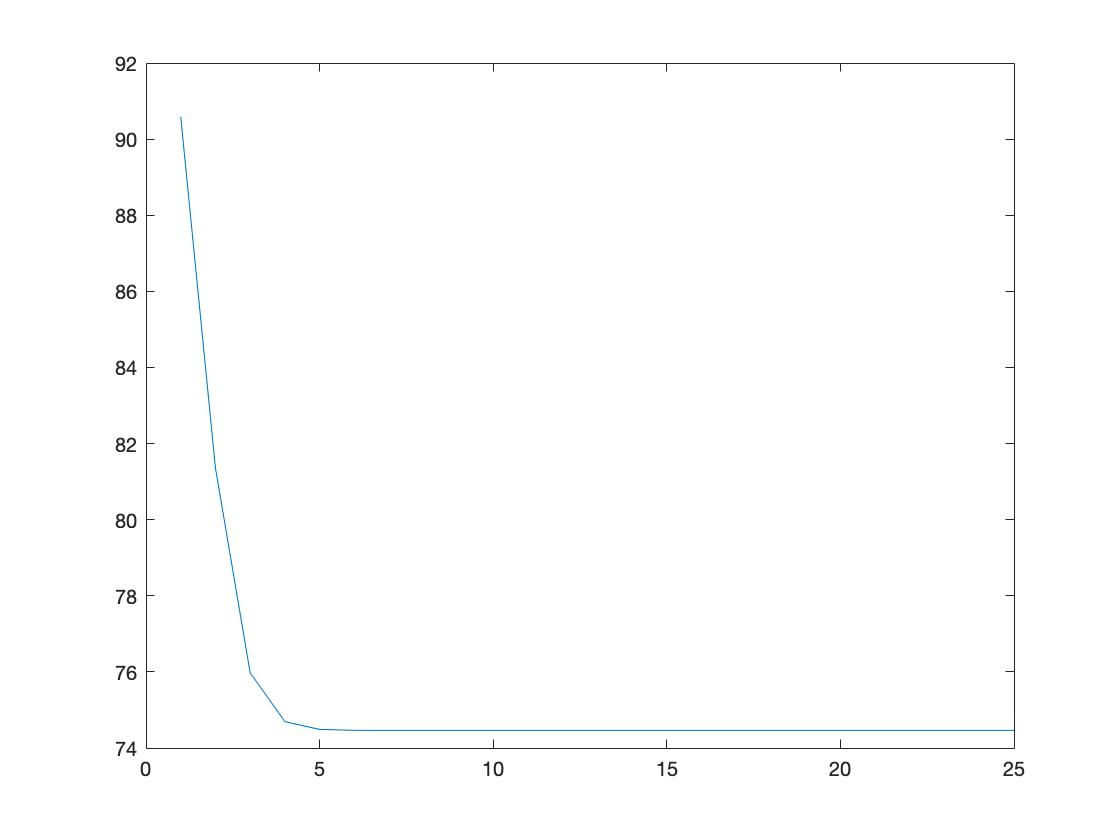
\includegraphics[scale=0.3]{trace.jpg}
\caption{trace of $\Sigma_t$ over frames}
\label{fig:label}
\end{figure}
From figure1 we can find that the trace of the covariance matrix converges to a relative small value.
\subsubsection*{Rotation matrix of each frame}
\par
See the rotation matrix in the Rotation.txt
\subsubsection*{3D structure of the object}
\par 
In this project, I choose the left up corner to be the origin of the object frame. And the 3D coordinates are as follow
\begin{equation*}
\begin{bmatrix}
0&10.586&75.685&-7.960&-23.283&-25.169&59.501&-48.330&26.307\\
0&-4.360&-21.182&-112.444&-133.398&-145.584&-169.7769&-193.930&-206.392\\
0&5.333&19.163&-37.087&-41.038&-48.369&-22.298&86.783&97.138
\end{bmatrix}
\end{equation*} 
\begin{figure}[H]
\centering
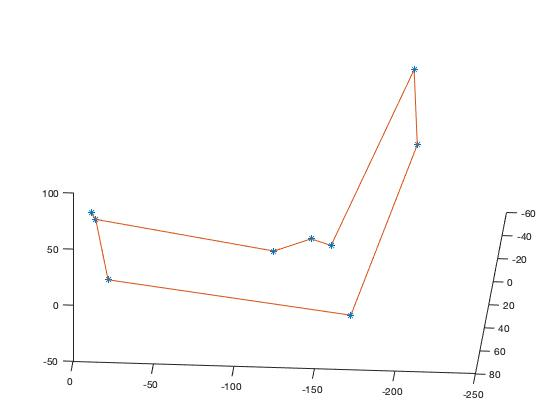
\includegraphics[scale=0.5]{3D_structure.jpg}
\caption{3D structure}
\label{fig:label}
\end{figure}
\subsection*{Conclusion and summary}
In this project I applied Kalman filter to track the feature points from frame to frame. And after getting all the points' 2D coordinates, I recovered the camera's rotation relative to the object frame and the 3D coordinates of the feature points using the factorization method.

\newpage

\begin{thebibliography}{}  
\bibitem{ref1}Qiang Ji. RPI ECSE 6650 Computer Vision, Lecture Notes: Motion. URL:https://www.ecse.rpi.edu/\~qji/CV/motion2.pdf. Last visited on 2019/12/8.
\end{thebibliography}
\end{document}